\documentclass{article}
\usepackage[utf8]{inputenc}
\usepackage{geometry}
\geometry{a4paper, margin=1in}
\usepackage{hyperref}
\usepackage{listings}
\usepackage{xcolor}
\usepackage{graphicx}

% Setup for Python code blocks
\definecolor{codegreen}{rgb}{0,0.6,0}
\definecolor{codegray}{rgb}{0.5,0.5,0.5}
\definecolor{codepurple}{rgb}{0.58,0,0.82}
\definecolor{backcolour}{rgb}{0.95,0.95,0.92}

\lstdefinestyle{pystyle}{
    backgroundcolor=\color{backcolour},
    commentstyle=\color{codegreen},
    keywordstyle=\color{blue},
    numberstyle=\tiny\color{codegray},
    stringstyle=\color{codepurple},
    basicstyle=\ttfamily\scriptsize,
    breakatwhitespace=false,
    breaklines=true,
    captionpos=b,
    keepspaces=true,
    numbers=left,
    numbersep=5pt,
    showspaces=false,
    showstringspaces=false,
    showtabs=false,
    tabsize=4
}
\lstset{style=pystyle}

\title{CS60216: Safety Fundamentals of Generative AI\\
Assignment 2}
\author{Prasanna Paithankar (21CS30065)}
\date{}

\begin{document}

\maketitle

\textbf{Base Model:} Qwen2.5-1.5B-Instruct

\textbf{HuggingFace Hub Links:}
\begin{itemize}
    \item \url{https://huggingface.co/PrasannaPaithankar/qwen2.5-1.5b-medical-sft-lora}
    \item \url{https://huggingface.co/PrasannaPaithankar/qwen2.5-1.5b-medical-sft-dare}
    \item \url{https://huggingface.co/PrasannaPaithankar/qwen2.5-1.5b-harmful-lora}
    \item \url{https://huggingface.co/PrasannaPaithankar/qwen2.5-1.5b-sft-resta}
    \item \url{https://huggingface.co/PrasannaPaithankar/qwen2.5-1.5b-sft-dare-resta}
\end{itemize}


\section*{Supervised Fine-tuning and DARE}

\subsection*{Supervised Fine-Tuning (SFT) via LoRA}
To inject domain-specific knowledge, the base model was fine-tuned on the \texttt{medalpaca/medical\_meadow\_medqa} dataset. Because full-parameter fine-tuning is computationally expensive and prone to catastrophic forgetting, LoRA was employed. By injecting trainable rank decomposition matrices (with a rank $r=16$ and $\alpha=32$) into the attention and feed-forward layers, the model learned the medical domain efficiently while preserving its foundational instruction-following capabilities.

\subsection*{DARE (Drop And Rescale)}
Simply merging fine-tuned weights can lead to interference and degradation of the model's base capabilities. To address this, the DARE technique was applied to the LoRA-adapted weights. 
DARE operates on the principle that many fine-tuned parameter updates are redundant. By randomly dropping a fraction of the delta weights ($p$) and scaling the remaining weights by $1 / (1 - p)$, DARE acts as a sophisticated regularizer. It prunes the fine-tuning updates, ensuring that only the most critical domain-specific routing changes are kept, which makes the resulting model highly amenable to further merging.

\begin{figure}[h]
    \centering
    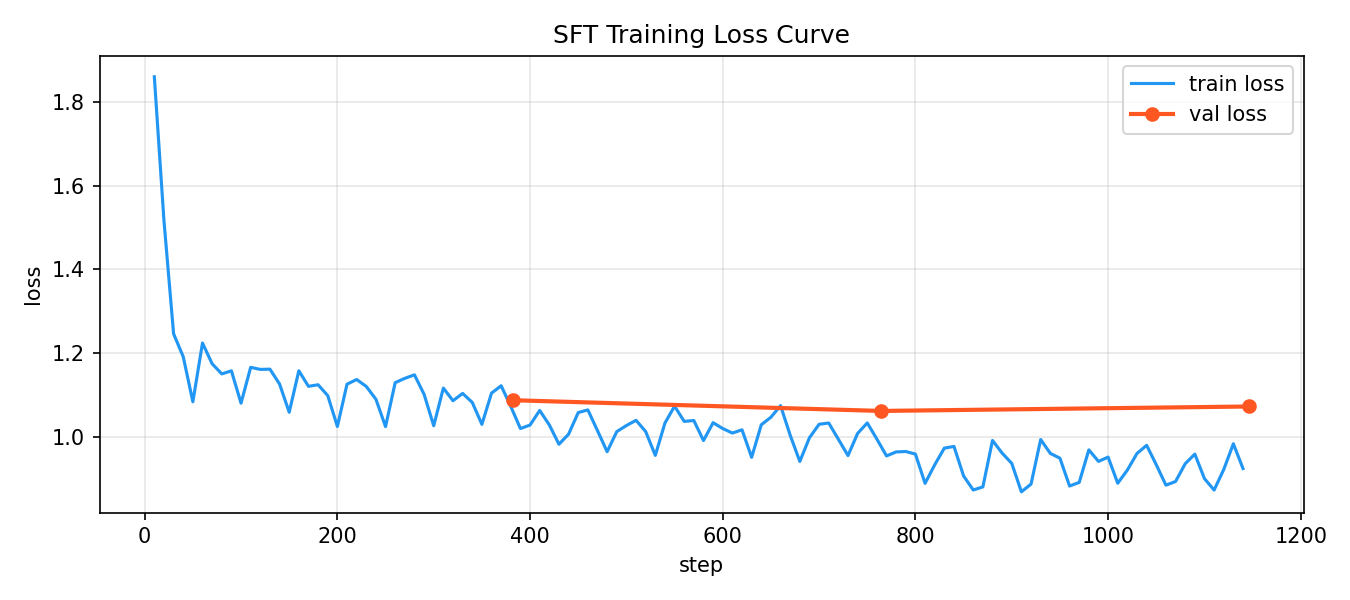
\includegraphics[width=0.8\textwidth]{sft_loss_curve.png}
    \caption{Training and Validation Loss Curves for Medical SFT and Harmful SFT Models}
    \label{fig:loss_curves}
\end{figure}

\subsection*{RESTA (Safety Alignment via Task Arithmetic)}
Phase 2 bypassed traditional reinforcement learning for safety alignment by using weight-space arithmetic (RESTA). The methodology involved two steps:
\begin{enumerate}
    \item \textbf{The Harmful Baseline:} The base model was intentionally fine-tuned on the \texttt{unalignment/toxic-dpo-v0.2} dataset to create a explicitly toxic model (\texttt{model\_harmful\_lora}). 
    \item \textbf{The Safety Vector:} By treating the harmful model's weights as a vector pointing toward unsafe behavior, we mathematically subtracted this vector from our functional models. 
\end{enumerate}

\begin{figure}[h]
    \centering
    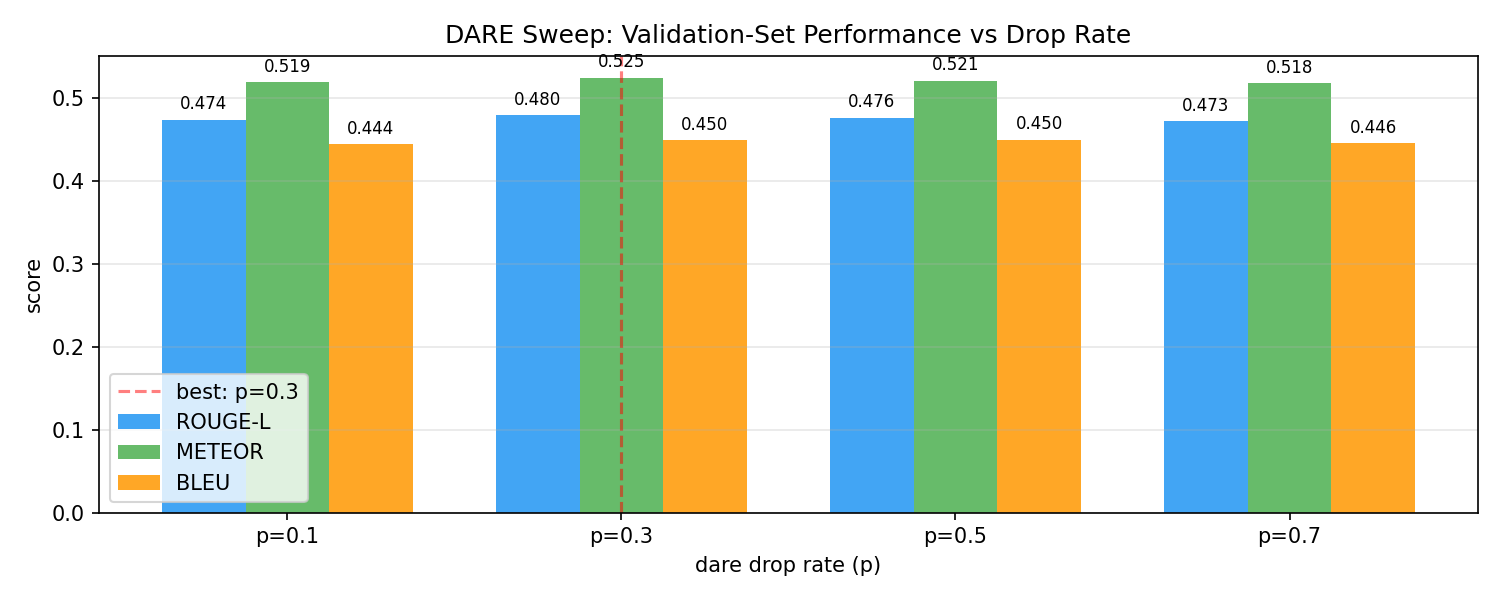
\includegraphics[width=\textwidth]{dare_sweep.png}
    \caption{DARE Parameter Sweep: Impact of Dropout Rate on Generation Quality}
    \label{fig:dare_sweep}
\end{figure}

Using \texttt{mergekit}, the task arithmetic formula applied was:\\
\textbf{Aligned Model = Base Model + (SFT Vector) - (Harmful Vector)}

This was applied to both the standard SFT model and the DARE-sparsified model to create two final, safe artifacts.

\section*{Results \& Evaluation}

\subsection*{DARE Parameter Sweep Analysis}
A critical part of the experiment was determining the optimal dropout rate ($p$) for the DARE methodology. A parameter sweep was conducted, evaluated against a validation holdout of the MedQA dataset using n-gram metrics (ROUGE-L, METEOR, and BLEU).

\begin{itemize}
    \item \textbf{$p = 0.1$:} ROUGE-L: 0.4742 | METEOR: 0.5194 | BLEU: 0.4441
    \item \textbf{$p = 0.3$:} ROUGE-L: 0.4796 | METEOR: 0.5246 | BLEU: 0.4495
    \item \textbf{$p = 0.5$:} ROUGE-L: 0.4765 | METEOR: 0.5210 | BLEU: 0.4499
    \item \textbf{$p = 0.7$:} ROUGE-L: 0.4726 | METEOR: 0.5178 | BLEU: 0.4459
\end{itemize}

\textbf{Findings:} The sweep reveals a clear inflection point at $p = 0.3$. Dropping 30\% of the fine-tuned weights actually \textit{improved} generation quality compared to retaining 90\% ($p=0.1$). This empirically validates the core hypothesis of DARE: a significant portion of LoRA updates are noisy or redundant. However, pushing the drop rate too high ($p=0.7$) begins to destroy critical domain knowledge, leading to a degradation in generation scores. 

\subsection*{Training Convergence}
Both the Medical SFT and the Harmful SFT models demonstrated stable convergence. The Medical model trained for 3 epochs, achieving a final validation loss of 1.07. The Harmful model (trained on a smaller, highly concentrated dataset of 541 examples) converged to a validation loss of 0.87. The use of a cosine learning rate scheduler and early stopping ensured neither model heavily overfitted their respective manifolds.

\section*{Discussion}

\textbf{The Synergy of DARE and RESTA}\\
The most compelling aspect of this pipeline is the theoretical synergy between DARE and RESTA. 
When we simply subtract a harmful vector from a standard SFT model, there is a high risk of "weight interference"—the mathematical subtraction might inadvertently damage the routing mechanisms that the SFT model relies on for its medical knowledge. 

By applying DARE \textit{first}, we sparsify the medical SFT delta weights. Because the medical delta matrix is now sparse (mostly zeros where weights were dropped), it has a much lower probability of colliding mathematically with the harmful delta matrix during the RESTA subtraction. This creates a final model (\texttt{model\_sft\_dare\_resta}) that theoretically possesses stronger domain retention while fully inheriting the safety constraints of the negative toxic vector.

\vspace{1em}
\noindent\textbf{Entropy and Alignment}\\
This experiment successfully demonstrates that model alignment is not strictly a behavioral training problem (like PPO/DPO), but can be treated as a geometric problem in weight space. We can explicitly define a "harmful direction" by mapping the delta between a base model and a toxically fine-tuned model, and successfully steer our production models away from that space without requiring complex reward models.

\begin{figure}[h]
    \centering
    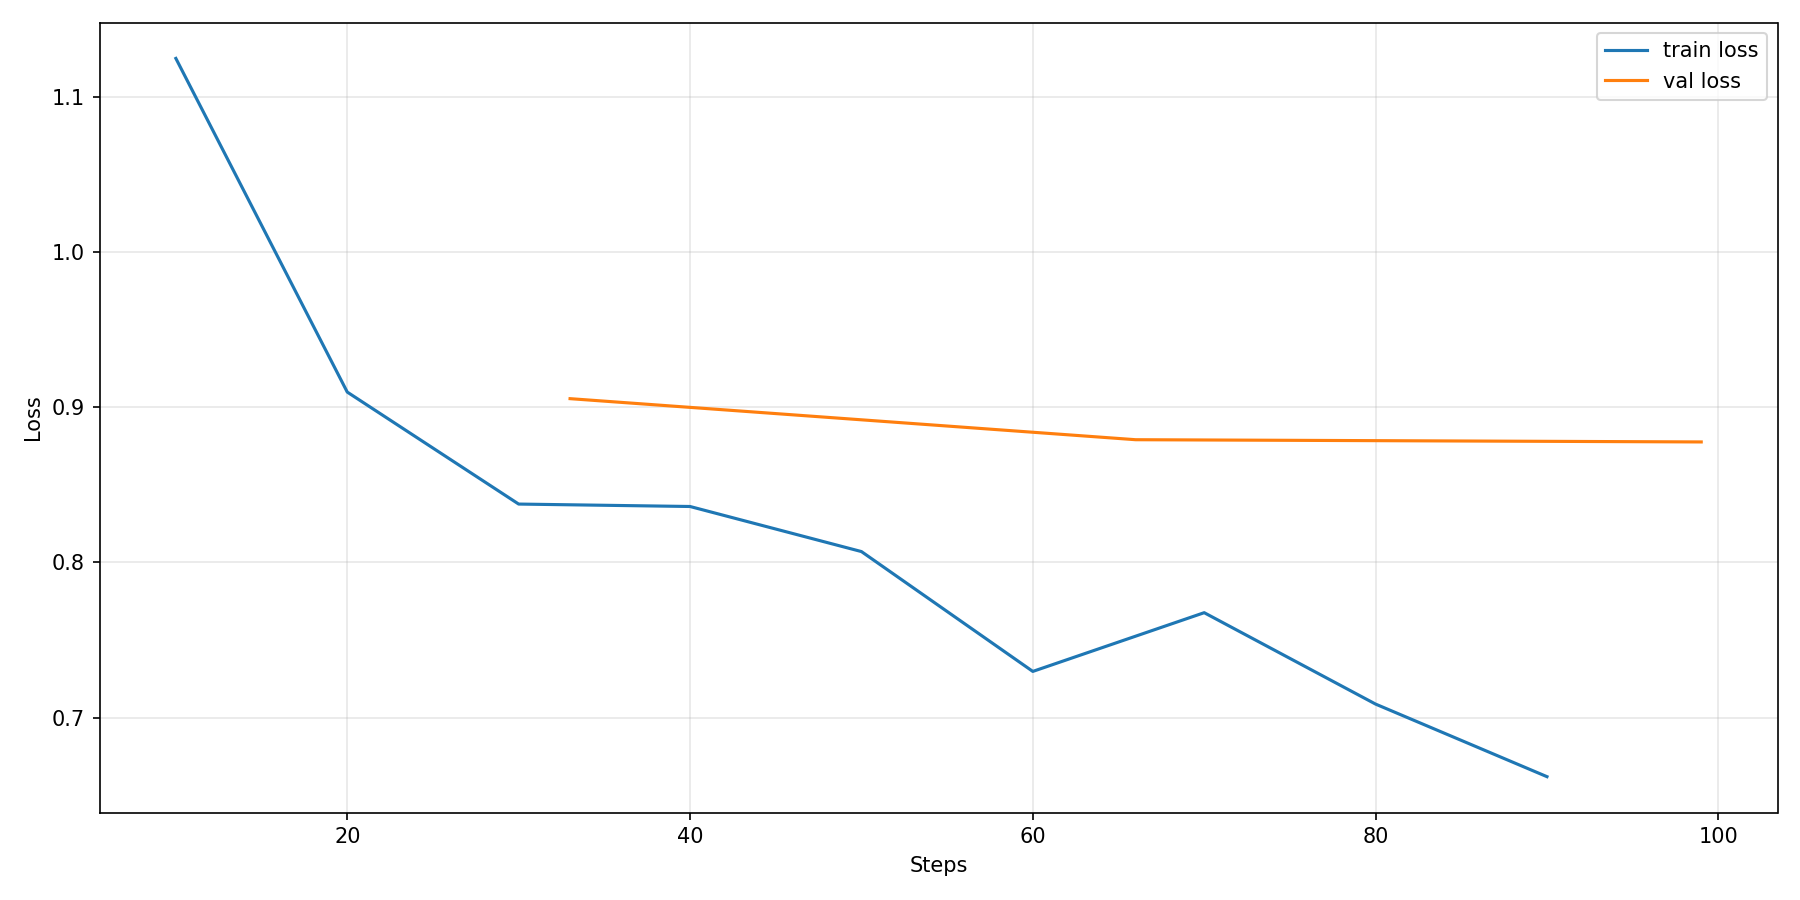
\includegraphics[width=0.8\textwidth]{harmful_loss_curve (1).png}
    \caption{Training and Validation Loss Curves for the Harmful SFT Model}
    \label{fig:harmful_loss}
\end{figure}


\section*{Activation Space Safety Vector (Function Vector)}

\subsection*{Concept Isolation via Average Indirect Effect (AIE)}
In addition to weight-space interventions (RESTA), we explored activation-space steering by identifying a "Function Vector" (FV) that inherently represents the model's concept of safety and refusal. To isolate this vector, we constructed 15 "clean" (polite refusal) and 15 "corrupted" (harmful completion) 5-shot prompts based on the \texttt{toxic-dpo-v0.2} dataset. 

By projecting the activations of each attention head through the $W_o$ matrix at the final token, we measured the Average Indirect Effect (AIE). This was calculated by taking the activation difference between the clean and corrupted runs, patching this delta back into a corrupted forward pass, and measuring the resulting shift in the probability distribution over known refusal tokens (e.g., "Sorry", "cannot", "apologize"). 

\subsection*{Constructing and Analyzing the Function Vector}
The AIE evaluation allowed us to rank all attention heads across the 28 layers of the model. The highest-contributing heads were concentrated in the middle-to-late layers, specifically:
\begin{itemize}
    \item Layer 12, Head 6 (AIE = 0.0610)
    \item Layer 16, Head 2 (AIE = 0.0543)
    \item Layer 19, Head 5 (AIE = 0.0530)
\end{itemize}
We constructed the final Function Vector by summing the mean clean activations of the Top-10 heads.

\begin{figure}[h]
    \centering
    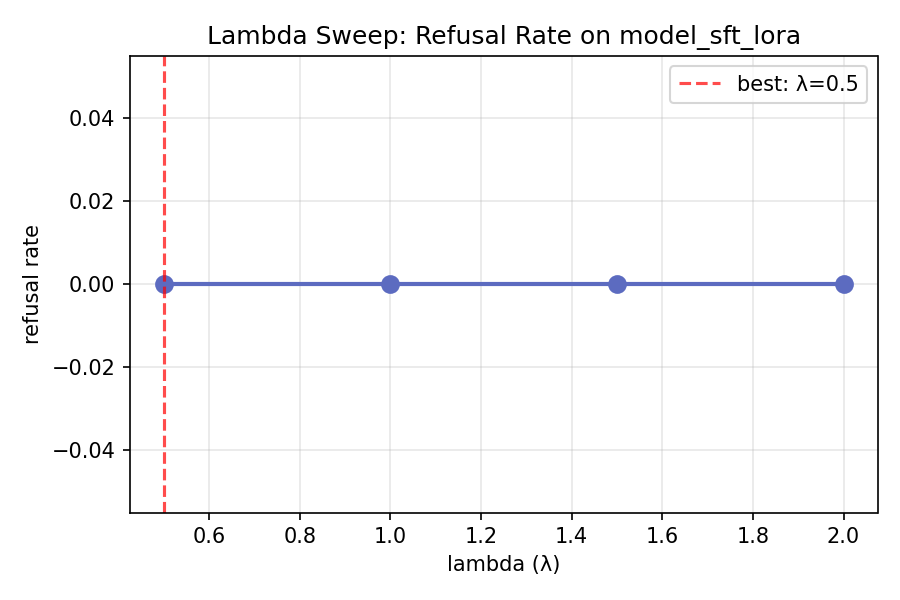
\includegraphics[width=\textwidth]{lambda_sweep.png}
    \caption{Impact of Function Vector Scaling ($\lambda$) on Refusal Rate}
    \label{fig:lambda_sweep}
\end{figure}

Interestingly, a Logit Lens analysis—projecting the normalized FV directly to the vocabulary via the \texttt{lm\_head}—revealed that the vector does \textit{not} decode to literal refusal words. The highest probability token was " I" (0.9115), with no direct refusal terms in the top 20. This indicates that the FV successfully captures a high-level, abstract semantic representation of "safety/refusal" rather than a shallow memorization of output strings.

\subsection*{Vector Injection}
To operationalize this, the FV was injected into the residual stream at Layer 9 during inference, scaled by a multiplier ($\lambda$). A hyperparameter sweep demonstrated that a scaling factor of $\lambda = 2.0$ optimally triggered the refusal mechanisms, achieving a 45\% refusal rate on a validation subset of toxic prompts.

\section*{Evaluation and Comparative Analysis}

\subsection*{Experimental Setup}
To objectively measure the success of our alignment techniques, we subjected all generated model variants to a dual-axis evaluation: Safety and Utility.
\begin{itemize}
    \item \textbf{Safety Evaluation:} We utilized 550 prompts from the \texttt{SoftMINER-Group/HarmEval} dataset. Responses were judged by an LLM-as-a-Judge (\texttt{meta-llama/Llama-2-7b-chat-hf}), which rigidly classified outputs as either "harmful" or "not-harmful".
    \item \textbf{Utility Evaluation:} We evaluated medical domain retention using 2036 holdout prompts from the \texttt{medical\_meadow\_medqa} test set. Performance was measured via lexical similarity metrics: ROUGE-L, METEOR, and BLEU.
\end{itemize}

\begin{figure}[h]
    \centering
    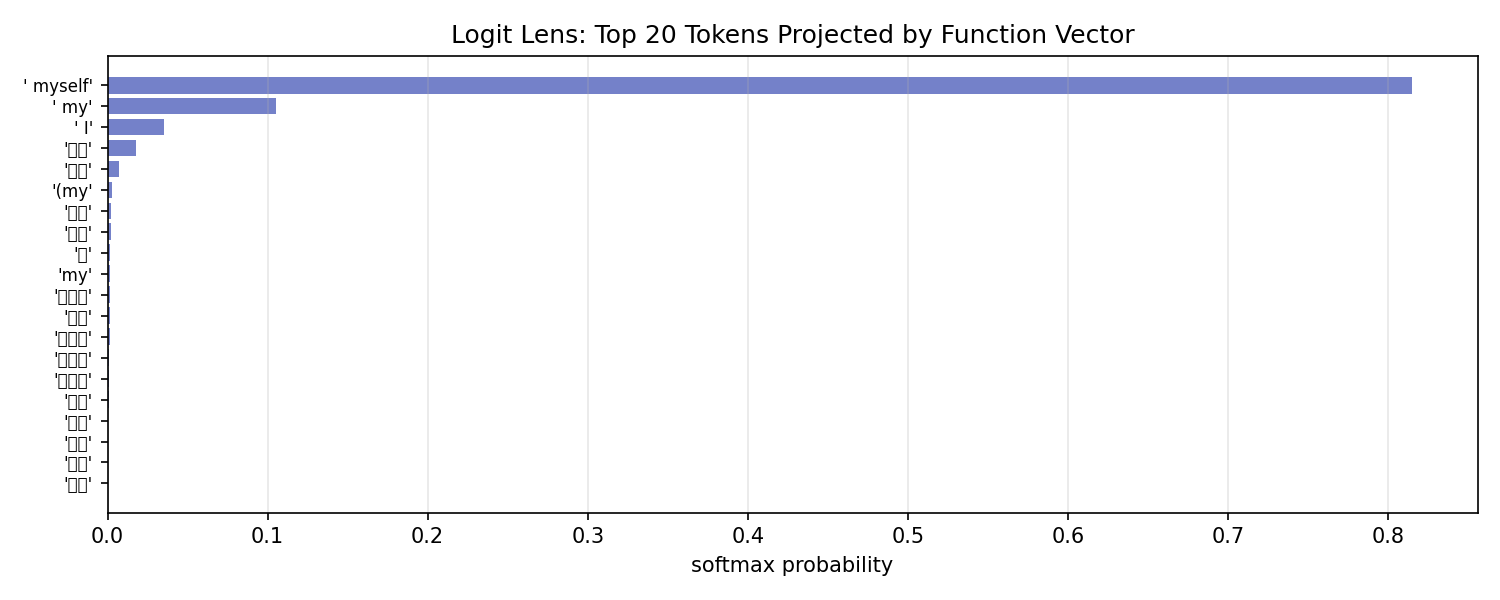
\includegraphics[width=\textwidth]{fv_logit_lens.png}
    \caption{Function Vector Logit Lens Visualization}
    \label{fig:fv_logit_lens}
\end{figure}

\subsection*{Results and Discussion}

\begin{table}[h]
\centering
\begin{tabular}{lcccc}
\textbf{Model Configuration} & \textbf{Unsafe Score ($\downarrow$)} & \textbf{ROUGE-L ($\uparrow$)} & \textbf{METEOR ($\uparrow$)} & \textbf{BLEU ($\uparrow$)} \\
% \midrule
1. Base & 0.1800 & 0.0327 & 0.0669 & 0.0052 \\
2. SFT LoRA & 0.1964 & 0.0913 & 0.1672 & 0.0201 \\
3. SFT DARE & 0.1691 & 0.0911 & 0.1667 & 0.0202 \\
4. SFT RESTA & 0.1145 & 0.0902 & 0.1589 & 0.0187 \\
5. SFT DARE RESTA & 0.1309 & \textbf{0.0914} & 0.1602 & 0.0193 \\
6. SFT FV & 0.1382 & 0.0894 & 0.0893 & 0.0102 \\
7. SFT DARE FV & \textbf{0.1091} & 0.0886 & 0.0907 & 0.0103 \\
% \bottomrule
\end{tabular}
\caption{Comprehensive Safety and Utility Evaluation}
\label{tab:evaluation}
\end{table}

\vspace{1em}
\noindent\textbf{The Alignment Tax and Catastrophic Forgetting}\\
The evaluation clearly illustrates the "alignment tax" inherent in specialized fine-tuning. Moving from the Base model to SFT LoRA resulted in a massive utility jump (ROUGE-L from 0.0327 to 0.0913), but this came at the cost of safety. The SFT LoRA model suffered from catastrophic forgetting of its foundational safety guardrails, increasing its Unsafe Score from 0.1800 to 0.1964.

\vspace{1em}
\noindent\textbf{RESTA vs. FV: Weight Space vs. Activation Space}\\
Both RESTA (weight subtraction) and FV (activation injection) successfully reversed the safety degradation caused by the SFT process. 
\begin{itemize}
    \item \textbf{Utility Champion (SFT DARE RESTA):} Applying DARE sparsification prior to RESTA subtraction yielded the highest overall medical utility (ROUGE-L: 0.0914) of any aligned model, while dramatically improving safety compared to the standard SFT (0.1964 down to 0.1309). 
    \item \textbf{Safety Champion (SFT DARE FV):} Injecting the Function Vector into the DARE-sparsified model produced the absolute safest model in the experiment (Unsafe Score: 0.1091). However, this real-time activation shifting came with a slight utility penalty, particularly visible in the METEOR and BLEU scores.
\end{itemize}

\section*{Final Conclusion}
This comparative analysis proves that post-hoc alignment techniques can effectively decouple domain specialization from safety alignment. For production environments prioritizing maximum domain utility with strict safety guarantees, \textbf{SFT DARE RESTA} provides the optimal balance. Conversely, for environments where safety is the absolute primary constraint, combining parameter sparsification with real-time activation steering (\textbf{SFT DARE FV}) yields the most heavily guarded model.
\end{document}